% This file was created with tikzplotlib v0.10.1.
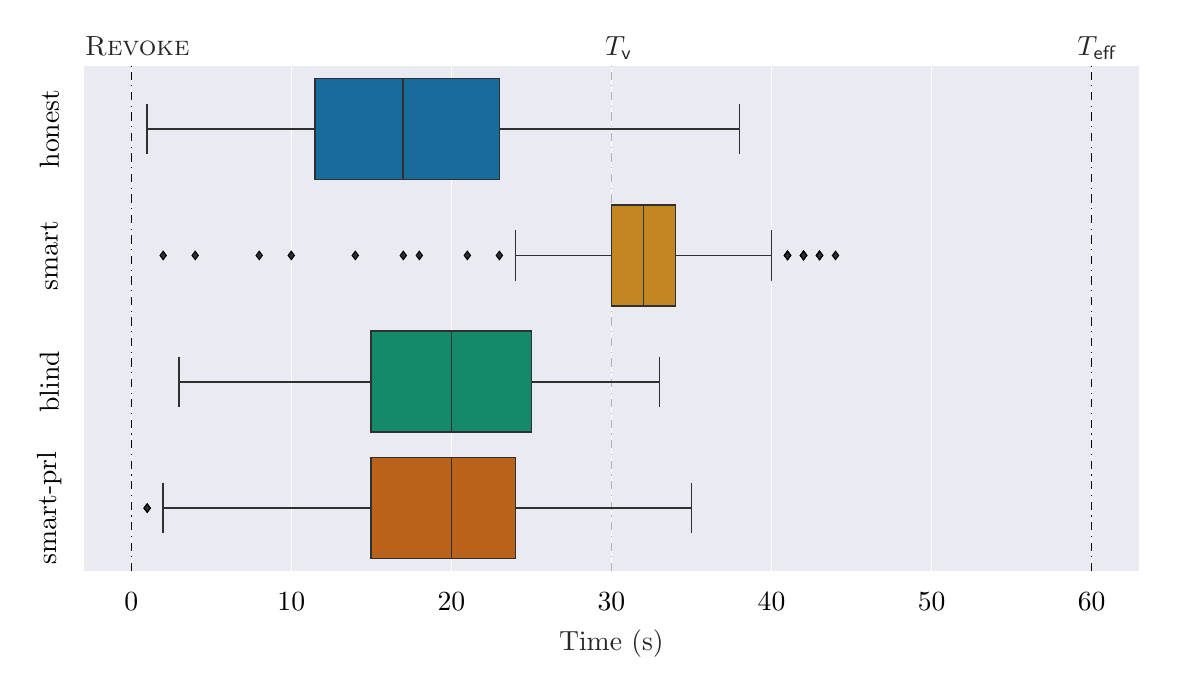
\begin{tikzpicture}

\definecolor{chocolate1869726}{RGB}{186,97,26}
\definecolor{darkgoldenrod19413532}{RGB}{194,135,32}
\definecolor{darkslategray38}{RGB}{38,38,38}
\definecolor{darkslategray48}{RGB}{48,48,48}
\definecolor{lavender234234242}{RGB}{234,234,242}
\definecolor{seagreen21138106}{RGB}{21,138,106}
\definecolor{teal23108155}{RGB}{23,108,155}

\begin{axis}[
clip=false,
axis background/.style={fill=lavender234234242},
axis line style={white},
height=8cm,
minor xtick={},
minor ytick={},
tick align=outside,
width=15cm,
x grid style={white},
xlabel=\textcolor{darkslategray38}{Time (s)},
xmajorgrids,
xmajorticks=true,
xmin=-3, xmax=63,
xtick style={color=darkslategray38,draw=none},
xtick={-10,0,10,20,30,40,50,60,70},
y dir=reverse,
y grid style={white},
ymajorticks=true,
ymin=-0.5, ymax=3.5,
ytick style={color=darkslategray38,draw=none},
ytick={0,1,2,3},
yticklabel style={rotate=90.0,anchor=center,yshift=8pt},
yticklabels={honest,smart,blind,smart-prl}
]
% START VERTICAL LINES %
\addplot [dashdotted, black]
table {%
0 3.5
0 -0.5
};
\addplot [dashdotted, gray!60]
table {%
30 3.5
30 -0.5
};
\addplot [dashdotted, black]
table {%
60 3.5
60 -0.5
};
% END VERTICAL LINES %
\path [draw=darkslategray48, fill=teal23108155, semithick]
(axis cs:11.5,-0.4)
--(axis cs:11.5,0.4)
--(axis cs:23,0.4)
--(axis cs:23,-0.4)
--(axis cs:11.5,-0.4)
--cycle;
\path [draw=darkslategray48, fill=darkgoldenrod19413532, semithick]
(axis cs:30,0.6)
--(axis cs:30,1.4)
--(axis cs:34,1.4)
--(axis cs:34,0.6)
--(axis cs:30,0.6)
--cycle;
\path [draw=darkslategray48, fill=seagreen21138106, semithick]
(axis cs:15,1.6)
--(axis cs:15,2.4)
--(axis cs:25,2.4)
--(axis cs:25,1.6)
--(axis cs:15,1.6)
--cycle;
\path [draw=darkslategray48, fill=chocolate1869726, semithick]
(axis cs:15,2.6)
--(axis cs:15,3.4)
--(axis cs:24,3.4)
--(axis cs:24,2.6)
--(axis cs:15,2.6)
--cycle;
\addplot [semithick, darkslategray48]
table {%
11.5 0
1 0
};
\addplot [semithick, darkslategray48]
table {%
23 0
38 0
};
\addplot [semithick, darkslategray48]
table {%
1 -0.2
1 0.2
};
\addplot [semithick, darkslategray48]
table {%
38 -0.2
38 0.2
};
\addplot [semithick, darkslategray48]
table {%
30 1
24 1
};
\addplot [semithick, darkslategray48]
table {%
34 1
40 1
};
\addplot [semithick, darkslategray48]
table {%
24 0.8
24 1.2
};
\addplot [semithick, darkslategray48]
table {%
40 0.8
40 1.2
};
\addplot [black, mark=diamond*, mark size=1.5, mark options={solid,fill=darkslategray48}, only marks]
table {%
2 1
23 1
10 1
18 1
14 1
4 1
8 1
17 1
21 1
44 1
43 1
41 1
42 1
41 1
42 1
43 1
41 1
43 1
42 1
42 1
};
\addplot [semithick, darkslategray48]
table {%
15 2
3 2
};
\addplot [semithick, darkslategray48]
table {%
25 2
33 2
};
\addplot [semithick, darkslategray48]
table {%
3 1.8
3 2.2
};
\addplot [semithick, darkslategray48]
table {%
33 1.8
33 2.2
};
\addplot [semithick, darkslategray48]
table {%
15 3
2 3
};
\addplot [semithick, darkslategray48]
table {%
24 3
35 3
};
\addplot [semithick, darkslategray48]
table {%
2 2.8
2 3.2
};
\addplot [semithick, darkslategray48]
table {%
35 2.8
35 3.2
};
\addplot [black, mark=diamond*, mark size=1.5, mark options={solid,fill=darkslategray48}, only marks]
table {%
1 3
1 3
};
\addplot [semithick, darkslategray48]
table {%
17 -0.4
17 0.4
};
\addplot [semithick, darkslategray48]
table {%
32 0.6
32 1.4
};
\addplot [semithick, darkslategray48]
table {%
20 1.6
20 2.4
};
\addplot [semithick, darkslategray48]
table {%
20 2.6
20 3.4
};
\draw (axis cs:-3.5,-0.58) node[
  scale=1,
  anchor=base west,
  text=darkslategray38,
  rotate=0.0
]{\textsc{Revoke}};
\draw[dashed] (axis cs:29,-0.58) node[
  scale=1,
  anchor=base west,
  text=darkslategray38,
  rotate=0.0
]{$T_{\mathsf{v}}$};
\draw (axis cs:58.5,-0.58) node[
  scale=1,
  anchor=base west,
  text=darkslategray38,
  rotate=0.0
]{$T_{\mathsf{eff}}$};
\end{axis}

\end{tikzpicture}
